%=====================
% Remove this after writing actual report
%=====================
%
%Maecenas sed ultricies felis. Sed imperdiet dictum arcu a egestas. 
%\begin{itemize}
%	\item Donec dolor arcu, rutrum id molestie in, viverra sed diam
%	\item Curabitur feugiat
%	\item turpis sed auctor facilisis
%	\item arcu eros accumsan lorem, at posuere mi diam sit amet tortor
%	\item Fusce fermentum, mi sit amet euismod rutrum
%	\item sem lorem molestie diam, iaculis aliquet sapien tortor non nisi
%	\item Pellentesque bibendum pretium aliquet
%\end{itemize}
%\blindtext
%
%Text requiring further explanation\footnote{Example footnote}.

%=====================
%  MATHEMATICS
%=====================
To accomplish our task, we implement a Support-Vector Machine. This method is used to separate data into two different classes by a hyperplane\footnote{A pivotal assumption in our application is that our data (the images of different digits) are indeed linearly separable. We will find that this is mostly true, but not 100\% so.}:
\begin{equation}
\vec{w}\cdot\vec{x} + b = 0
\end{equation}
The two sets' vectors with the minimum distance to each other are defined as the support vectors, and assigned a $y_{i}$ shift of $1$ or $-1$ from the separating hyperplane. These vectors form the two constraints on our optimal hyperplane:
\begin{equation}
\begin{gathered}
	\vec{w}\cdot\vec{x_0} + b \geq 1 \text{ , if } \vec{y_i} = 1 \\
	\vec{w}\cdot\vec{x_1} + b \leq -1 \text{ , if } \vec{y_i} = -1 
\end{gathered}
\end{equation}

Figure \ref{fig:SVM_fig2} shows this concept using a Matlab plot

\begin{figure*}[t]
	\begin{subfigure}[t]{0.5\textwidth}
		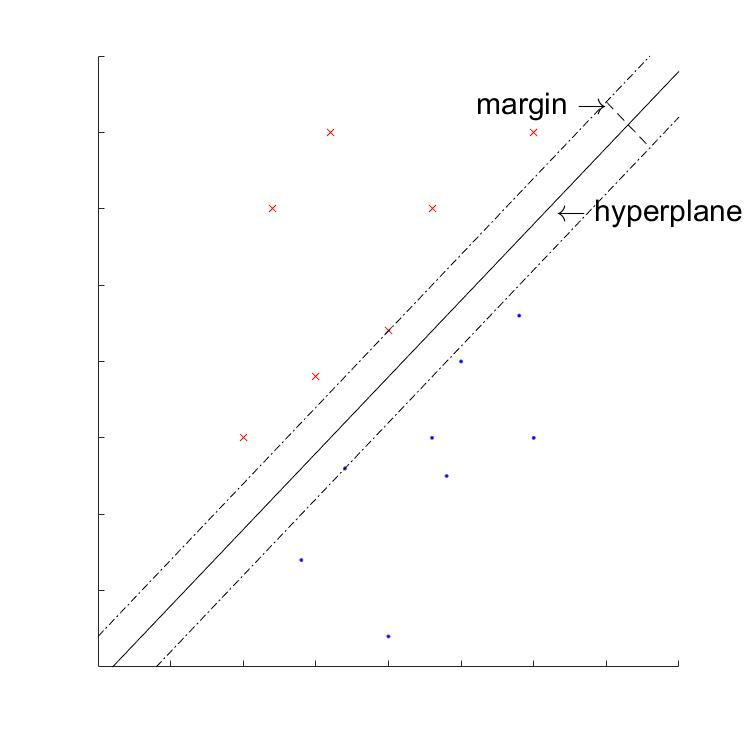
\includegraphics[width=7cm, height=7cm]{SVM_fig2}
		\caption{}
		\centering
		\label{fig:SVM_fig_a}
	\end{subfigure}%
	~
	\begin{subfigure}[t]{0.5\textwidth}
		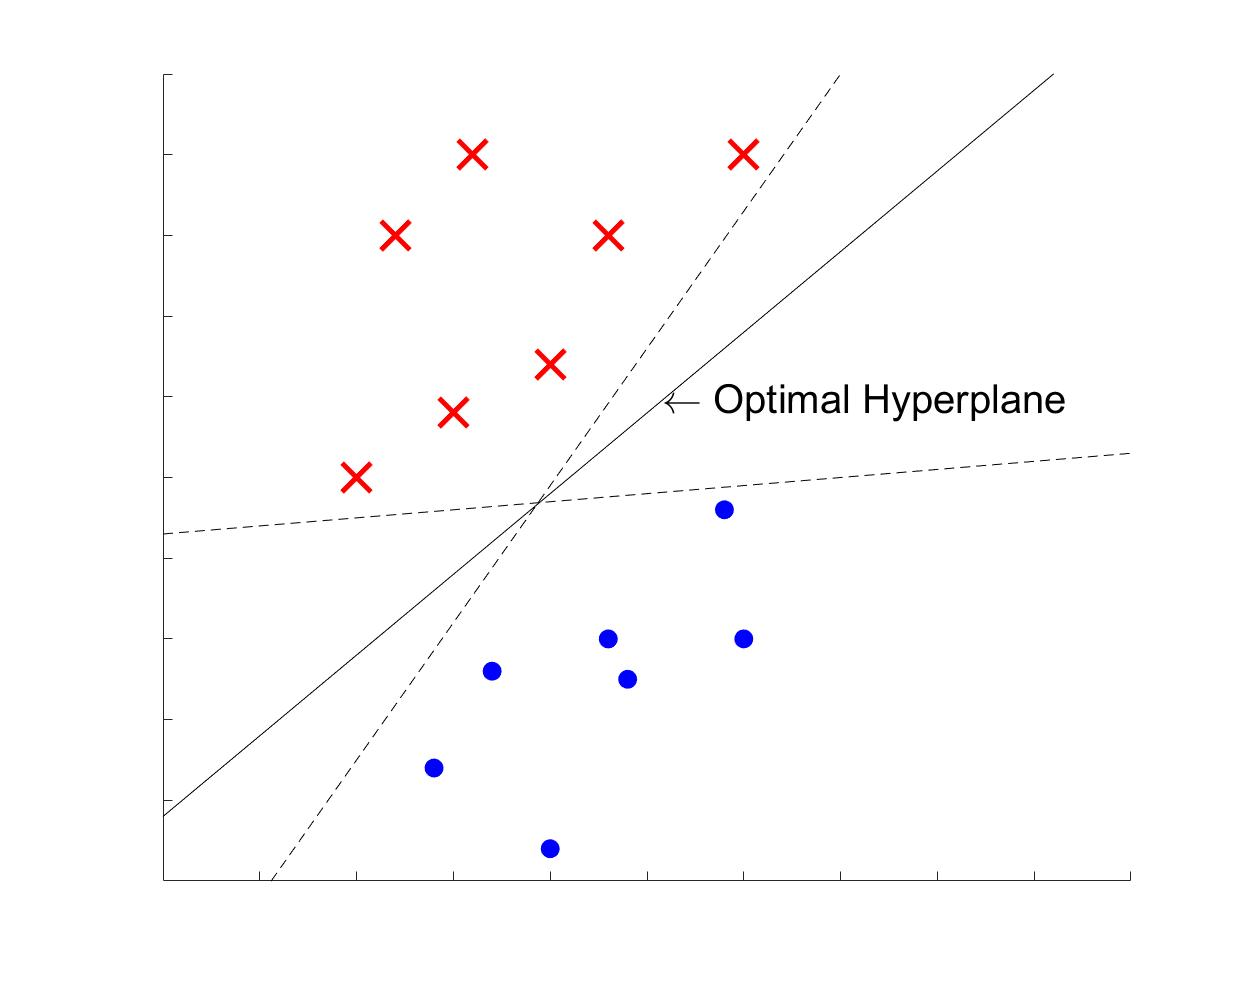
\includegraphics[width=7cm, 			height=7cm]{SVM_fig}
		\caption{}
		\centering
		\label{fig:SVM_fig_b}
	\end{subfigure}%
	
	\caption{The hyperplane is constrained to be within the limits of the margin, which are themselves defined by the support vectors.}
	\label{fig:SVM_fig}
\end{figure*}

This form is called canonical, as we have chosen to define $y \in \{-1, 1\}$. The choices of -1 and 1 are arbitrary, but result in the simplest most efficient calculation in computer applications. The set of $y$ values represents our two classes, and must always only have two elements. The problem of applying this to problems with more than 2 cases is discussed later, since our problem is to differentiate between 10 classes of numerical digits.
\subparagraph{A Note on the Fundamental Theorem of Linear Algebra}
This application represents the two classes as Class 1 and Not Class 1 (note the binary relationship). Therefore the two classes in this case must be orthogonal compliments to each other in the superspace they both reside. That is: the sum of the dimension of Class 1 and 2 must equal the superspace which they occupy. As an example on the superspace $V = \Re^3$, assume Class 1 is defined by the span of column vectors: 
\begin{equation}
V_{C_{1}} = 
span(\begin{pmatrix}
1 & 0 \\0 & 1\\1& 0
\end{pmatrix}),
\end{equation}

then Class two must be defined as:
\begin{equation}
V_{C_{2}} = span(\begin{pmatrix}
-1\\0\\1
\end{pmatrix}
)
\end{equation}

This is a trivial example, but he beauty of SVMs is that we can define these classes however we like -- as long as we can convert some set of objects into vectors.
\subparagraph{The Optimal Hyperplane}

The optimal hyperplane is defined as the plane that results in zero error and that maximizes the distance from the support vectors. Figure \ref{fig:SVM_fig} shows the optimal hyperplane perfectly in the middle of the two support-vector constraints. In our use of two canonical classes, this distance can be derived to be 
\begin{equation}
\frac{1}{2}\vec{w}\cdot\vec{w} = \frac{{||\vec{w}||}^2}{2}
\label{dist}
\end{equation}

 and this is shown in the Appendix.

We now have a maximization problem. Maximizing Equation \ref{dist} will optimize the margin of error of the separating plane and thus be the most accurate in determining which class any given input vector belongs to. 

\subparagraph{Linear Separability}
The accuracy of the SVM very much depends on the data. If the data is linearly separable, the SVM will be more accurate than a set that is not. This is because SVMs only use linear hyperplanes, meaning they cannot bend around outliers or fluctuations in data. With that said, a non-linearly separable dataset can be transformed into a linear dataset using what is called a kernel function. These functions are inherently nonlinear since if we were to have a linear transformation and tried to find a better hyperplane for the data $\vec{x}$:
\begin{equation}
\begin{gathered}
	L[\vec{x}] = A\vec{x} = \vec{x}^{'} \\
	\vec{w}\cdot \vec{x} \Rightarrow \vec{w} \cdot \vec{x}^{'} = \vec{w}A\vec{x} = \vec{w}^{'}\cdot\vec{x} 
\end{gathered}
\end{equation}

This is again a hyperplane on the same set $\vec{x}$, and provides us no better solution.

With a nonlinear kernal function, we can turn a set as in Figure \ref{fig:pre-trans} into a set as in Figure \ref{fig:post-trans}. This allows us to use linear hyperplanes with a non-linearly separable set of data.

\begin{figure*}[t]
	\centering
	\begin{subfigure}[t]{0.5\textwidth}
		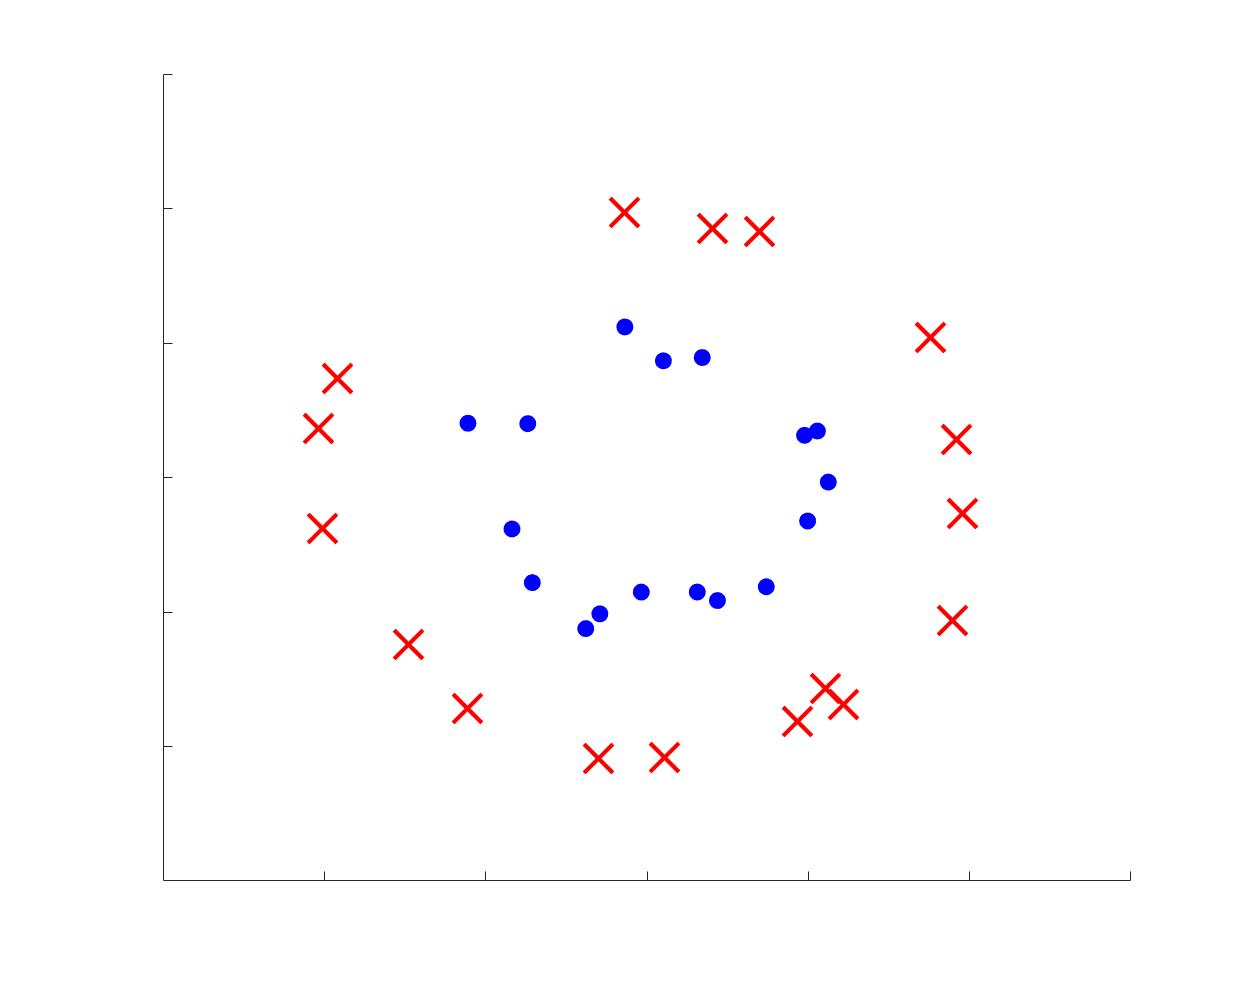
\includegraphics[width=7cm, height=7cm]{pre-transformation}
		\caption{}
		\centering
		\label{fig:pre-trans}
	\end{subfigure}%
~
	\begin{subfigure}[t]{0.5\textwidth}
		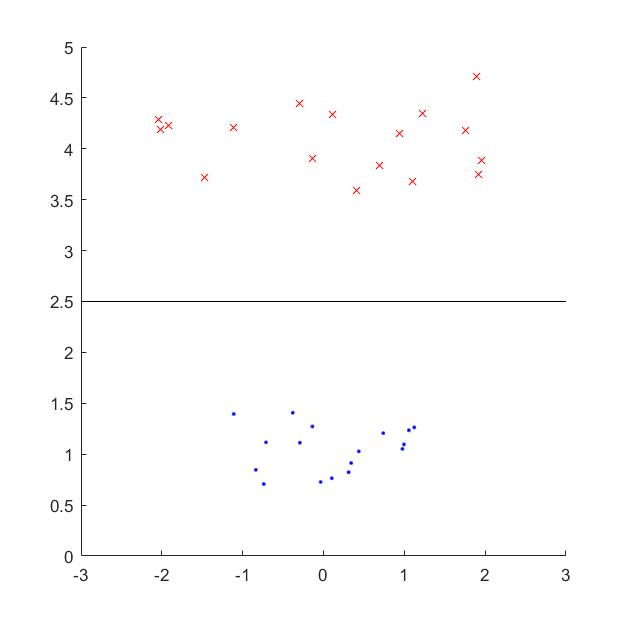
\includegraphics[width=7cm, 			height=7cm]{post-transform}
		\caption{}
		\centering
		\label{fig:post-trans}
	\end{subfigure}%

	\caption{The data before (\ref{fig:pre-trans}) and after (\ref{fig:post-trans}) a nonlinear kernal function was applied. It is now linearly separable and thus an SVM is a viable classifying tool. }	
	\label{fig:trans}
\end{figure*}
